\section{Surfaces Defined Parametrically and Surface Area} \label{S:11.6.Parametric_Surfaces_Surface_Area}

\vspace*{-14 pt}
\framebox{\hspace*{3 pt}
\parbox{6.25 in}{\begin{goals}
\item What is a parameterization of a surface?
\item How do we find the surface area of a parametrically defined surface?
\end{goals}} \hspace*{3 pt}}


\subsection*{Introduction}

We have now studied at length how curves in space can be defined parametrically by functions of the form $\vr(t) = \langle x(t), y(t), z(t) \rangle$, and surfaces can be represented by functions $z = f(x,y)$.  In what follows, we will see how we can also define surfaces parametrically.  A one-dimensional curve in space results from a vector function that relies upon one parameter, so a two-dimensional surface naturally involves the use of two parameters.  If $x = x(s, t)$, $y = y(s, t)$, and $z = z(s, t)$ are functions of independent parameters $s$ and $t$, then the terminal points of all vectors of the form
\[\vr(s, t) = x(s, t) \vi + y(s, t) \vj + z(s, t) \vk\]
form a surface in space. The equations $x=x(s,t)$, $y=y(s,t)$, and $z=z(s,t)$ are the \emph{parametric equations}\index{parameterization!surface} for the surface, or a \emph{parametrization} of the surface. In Preview Activity \ref{PA:11.6} we investigate how to parameterize a cylinder and a cone. 

\begin{pa} \label{PA:11.6} Recall the standard parameterization of the unit circle that is given by
\[x(t) = \cos(t) \ \ \ \ \text{ and } \ \ \ \ y(t) = \sin(t),\]
where $0 \le t \le 2\pi$.
    \ba
        \item Determine a parameterization of the circle of radius 1 in $\R^3$ that has its center at $(0,0,1)$ and lies in the plane $z=1$.

        \item Determine a parameterization of the circle of radius 1 in 3-space that has its center at $(0,0,-1)$ and lies in the plane $z=-1$.

        \item Determine a parameterization of the circle of radius 1 in 3-space that has its center at $(0,0,5)$ and lies in the plane $z=5$.

        \item Taking into account your responses in (a), (b), and (c), describe the graph that results from the set of parametric equations
        \[x(s,t) = \cos(t), \ \ \ \ y(s,t) = \sin(t), \ \ \ \ \text{ and } \ \ \ \ z(s,t) = s,\]
        where $0 \le t \le 2\pi$ and $-5 \le s \le 5$.         Explain your thinking.


    \item Just as a cylinder can be viewed as a ``stack'' of circles of constant radius, a cone can be viewed as a stack of circles with varying radius.  Modify the parametrizations of the circles above in order to construct the parameterization of a cone whose vertex lies at the origin, whose base radius is 4, and whose height is 3, where the base of the cone lies in the plane $z = 3$. Use appropriate technology\footnote{e.g., \url{http://www.flashandmath.com/mathlets/multicalc/paramrec/surf_graph_rectan.html}} to plot the parametric equations you develop. (Hint: The cross sections parallel to the $xz$ plane are circles, with the radii varying linearly as $z$ increases.)


    \ea
 
\end{pa} 
  
\begin{activitySolution}

    \ba
        \item A parameterization of the circle of radius 1 in $\R^3$ that has its center at $(0,0,1)$ and lies in the plane $z=1$ is
\[x(t) = \cos(t), \ y(t) = \sin(t), \ \text{ and } \ z(t) = 1.\]

        \item A parameterization of the circle of radius 1 in 3-space that has its center at $(0,0,-1)$ and lies in the plane $z=-1$ is
\[x(t) = \cos(t), \ y(t) = \sin(t), \ \text{ and } \ z(t) = -1.\]

        \item A parameterization of the circle of radius 1 in 3-space that has its center at $(0,0,5)$ and lies in the plane $z=5$.
\[x(t) = \cos(t), \ y(t) = \sin(t), \ \text{ and } \ z(t) = 5.\]

        \item This set of parametric equations would describe a cylinder centered around the $z$-axis, with a radius of $1$, that extended from $z=-5$ to $z=5$. The parameter $s$ in $z(t)$ allows the $z$ value to vary independently of the parameter $t$, which traces out the circles at each cross-sectional level of the cylinder.

    \item If we set the vertex of the cone at the origin and orient the cone to open upwards, then the cross sections parallel to the $xz$ plane are again circles, with the radii varying linearly as $z$ varies. So the parameterization defined by 
\[\vr(s,t) = t \cos(s) \vi + t \sin(s) \vj + t \vk\]
for $t \geq 0$ will gives us a cone.

If we want a cone with base radius 4 and height 3, we can modify the equations a bit. We need the radii to increase linearly so that when $z$ is 3 the radius of the cross section parallel to the $xy$ plane is 4. That means we need the radii to be $\frac{4}{3}z$ as $z$ increases from 0 to 3. So a parameterization that will gives us this cone is defined by
\[\vr(s,t) = \frac{4}{3}t \cos(s) \vi + \frac{4}{3} t \sin(s) \vj + t \vk\]
for $t$ from 0 to 3.

    \ea


\end{activitySolution}    

\afterpa 

\subsection*{Parametric Surfaces}

%\begin{activity} \label{A:11.6.1} Recall how the Cartesian coordinates of a point are related to the spherical coordinates of a point. Use this relationship to find a two-variable parameterization of a sphere of radius 2. Draw the surface defined by your parameterization with appropriate technology (e.g., \url{http://web.monroecc.edu/manila/webfiles/calcNSF/JavaCode/CalcPlot3D.htm} or \url{http://www.flashandmath.com/mathlets/multicalc/paramrec/surf_graph_rectan.html}).



\end{activity}
\begin{smallhint}

\end{smallhint}
\begin{bighint}

\end{bighint}
\begin{activitySolution}
We have $x(\theta,\phi) = \rho \cos(\theta) \cos(\phi)$, $y(\theta,\phi) = \rho \sin(\theta) \cos(\phi)$, and $z(\theta,\phi) = \rho \sin(\phi)$. So if we let $\rho = 2$, this will give us a parameterization of the sphere of radius centered at the origin, for $0 \leq \theta \leq 2\pi$ and $0 \leq \phi \leq 2\pi$.

\end{activitySolution}
\aftera

In a single-variable setting, any function may have its graph expressed parametrically.  For instance, given $y = g(x)$, by considering the parameterization $\langle t, g(t) \rangle$ (where $t$ belongs to the domain of $g$), we generate the same curve.  What is more important is that certain curves that are not functions may be represented parametrically; for instance, the circle (which cannot be represented by a single function) can be parameterized by $\langle \cos(t), \sin(t) \rangle$, where $0 \le t \le 2\pi$.

In the same way, in a two-variable setting, the surface $z = f(x,y)$ may be expressed parametrically by considering 
$$\langle x(s,t), y(s,t), z(s,t) \rangle = \langle s, t, f(s,t) \rangle,$$
where $(s,t)$ varies over the entire domain of $f$.  Therefore, any familiar surface that we have studied so far can be generated as a parametric surface.  But what is more powerful is that there are surfaces that cannot be generated by a single function $z = f(x,y)$ (such as the unit sphere), but that can be represented parametrically.  We now consider an important example.


%\begin{activity} \label{A:11.6.2} Let $f = f(x,y)$ be a function of $x$ and $y$. Find a two-variable parameterization of the surface defined by $f$. This shows that any of our familiar surfaces can be drawn as parametric surfaces.

\end{activity}
\begin{smallhint}

\end{smallhint}
\begin{bighint}

\end{bighint}
\begin{activitySolution}

All we need to do is to let $x(s,t) = s$, $y(s,t) = y$, and $z(s,t) = f(s,t)$.


\end{activitySolution}
\aftera




\begin{example} \label{ex:11.6.Torus} Consider the 
  torus (or doughnut) shown in Figure \ref{F:11.6.torus}.

  \begin{figure}[ht]
    \begin{center}
      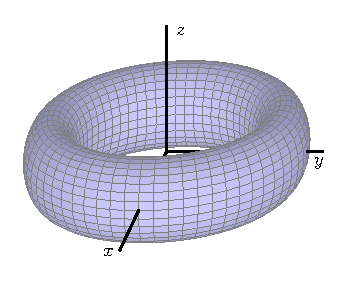
\includegraphics{figures/fig_11_6_torus.eps}
    \end{center}
    \caption{A torus}
    \label{F:11.6.torus}
  \end{figure}

To find a parametrization of this torus, we recall our work in Preview
Activity \ref{PA:11.6}.  There, we saw that a circle of radius $r$
that has its center at the point $(0,0,z_0)$ and is contained in the
horizontal plane $z = z_0$, as shown in Figure \ref{F:11.6.revolve}, can be
parametrized using the vector-valued function
$$
\vr(t) = r\cos(t)\vi + r\sin(t)\vj + z_0\vk
$$
where $0\leq t\leq 2\pi$.

\begin{figure}[ht]
  \begin{center}
    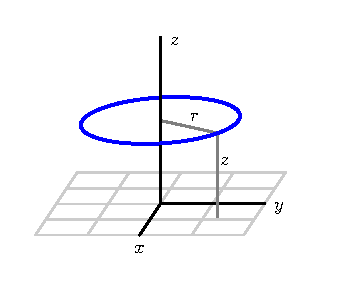
\includegraphics{figures/fig_11_6_revolve.eps}
  \end{center}
  \caption{A circle in a horizontal plane centered at $(0,0,z_0)$.}
  \label{F:11.6.revolve}
\end{figure}

To obtain the torus in Figure \ref{F:11.6.torus}, we begin with a circle of radius $a$ in the
$xz$-plane centered at $(b,0)$, as shown 
on the left of Figure \ref{F:11.6.torus.revolve}.  We may parametrize
the points on this circle, using the parameter $s$, by using the equations
$$
x(s) = b + a\cos(s)\hspace*{20pt}\mbox{and}\hspace*{20pt}
z(s) = a\sin(s),
$$
where $0\leq s \leq 2\pi$.  

\begin{figure}[ht]
  \begin{center}
    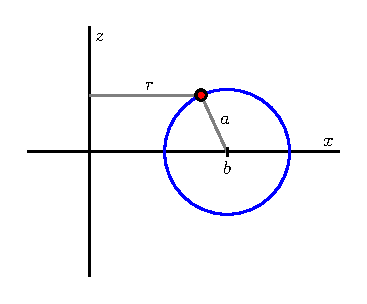
\includegraphics{figures/fig_11_6_torus_cross.eps}
    \hspace*{20pt}
    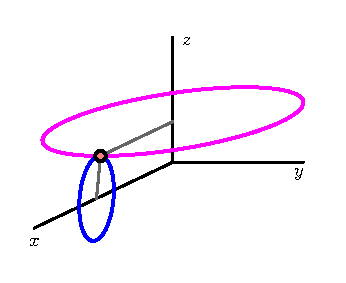
\includegraphics{figures/fig_11_6_torus_revolve.eps}
  \end{center}
  \caption{Revolving a circle to obtain a torus.}
  \label{F:11.6.torus.revolve}
\end{figure}

Let's focus our attention on one point on this circle, such as the
indicated point, which has coordinates $(x(s), 0, z(s))$
for a fixed value of the 
parameter $s$.  When this point is revolved about the $z$-axis, we
obtain a circle contained in a horizontal plane centered at
$(0,0,z(s))$ and having radius $x(s)$, as shown on the right of Figure
\ref{F:11.6.torus.revolve}.  If we let $t$ be the new parameter that generates the circle for the rotation about the $z$-axis, this circle may be
parametrized by
$$
\vr(s,t) = x(s)\cos(t)\vi + x(s)\sin(t)\vj + z(s)\vk.
$$
Now using our earlier parametric equations for $x(s)$ and $z(s)$ for the original smaller circle, we have an overall parameterization of the torus given by
$$
\vr(s,t) =(b+a\cos(s))\cos(t)\vi + 
(b+a\cos(s))\sin(t)\vj + 
a\sin(s)\vk.
$$
To trace out the entire torus, we require that the parameters vary through the values $0\leq s\leq 2\pi$ and
$0\leq t\leq 2\pi$.

\end{example}

%fig_11_6_approx.eps   fig_11_6_sphere_half.eps  
%fig_11_6_sphere.eps   

\begin{activity} \label{A:11.6.10}  In this activity, we seek a
  parametrization of the sphere of radius $R$ centered at the origin, as
  shown on the left in Figure \ref{F:11.6.sphere}.  
  Notice that this sphere may be obtained by revolving a half-circle
  contained in the $xz$-plane about the $z$-axis, as shown on the right.

  \begin{figure}[ht]
    \begin{center}
      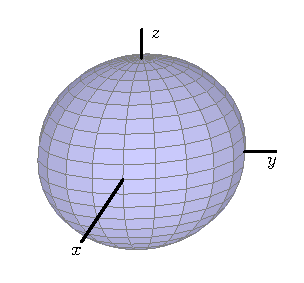
\includegraphics{figures/fig_11_6_sphere.eps}
      \hspace*{20pt}
      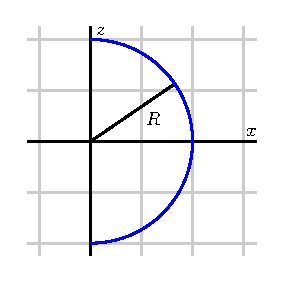
\includegraphics{figures/fig_11_6_sphere_half.eps}
    \end{center}
    \caption{A sphere obtained by revolving a half-circle.}
    \label{F:11.6.sphere}
  \end{figure}

  \ba
  \item Begin by writing a parametrization of this half-circle using
    the parameter $s$:
    $$
    x(s) = \ldots,\hspace*{20pt}
    z(s) = \ldots.
    $$
    Be sure to state the domain of the parameter $s$.
  \item By revolving the points on this half-circle about the
    $z$-axis, obtain a parametrization $\vr(s,t)$ of the points on the
    sphere of radius $R$.  Be sure to include the domain of both
    parameters $s$ and $t$. (Hint: What is the radius of the circle obtained when revolving a point on the half-circle around the $z$ axis?)

  \item Draw the surface defined by your parameterization with
    appropriate technology\footnote{e.g.,
    \url{http://web.monroecc.edu/manila/webfiles/calcNSF/JavaCode/CalcPlot3D.htm}
    or
    \url{http://www.flashandmath.com/mathlets/multicalc/paramrec/surf_graph_rectan.html}}.

    \ea



\end{activity}
\begin{smallhint}

\end{smallhint}
\begin{bighint}

\end{bighint}
\begin{activitySolution}
\ba
\item The parameterization of the half-circle is $x = R\cos(s)$, $y = 0$, $z=R\sin(s)$ for $-\frac{\pi}{2} \leq s \leq \frac{\pi}{2}$. 
\item A parameterization of the curve obtained by revolving the point $(R\cos(s), 0, R\sin(s))$ around the $z$-axis is $x=r\cos(t)$, $y=r\sin(t)$, $z=R\sin(s)$ for $0 \leq t \leq 2\pi$, where $r$ is the distance from the point to the $z$-axis. Note that this distance is just $R\cos(s)$, So a parameterization of the sphere of radius $R$ centered at the origin is 
\[\vr(s,t) = \langle R\cos(s)\cos(t), R\cos(s)\sin(t), R\sin(s) \rangle\]
for  $-\frac{\pi}{2} \leq s \leq \frac{\pi}{2}$ and $0 \leq t \leq 2\pi$. 
\ea

\end{activitySolution}
\aftera


%\begin{activity} \label{A:11.6.1} Recall how the Cartesian coordinates of a point are related to the spherical coordinates of a point. Use this relationship to find a two-variable parameterization of a sphere of radius 2. Draw the surface defined by your parameterization with appropriate technology (e.g., \url{http://web.monroecc.edu/manila/webfiles/calcNSF/JavaCode/CalcPlot3D.htm} or \url{http://www.flashandmath.com/mathlets/multicalc/paramrec/surf_graph_rectan.html}).



\end{activity}
\begin{smallhint}

\end{smallhint}
\begin{bighint}

\end{bighint}
\begin{activitySolution}
We have $x(\theta,\phi) = \rho \cos(\theta) \cos(\phi)$, $y(\theta,\phi) = \rho \sin(\theta) \cos(\phi)$, and $z(\theta,\phi) = \rho \sin(\phi)$. So if we let $\rho = 2$, this will give us a parameterization of the sphere of radius centered at the origin, for $0 \leq \theta \leq 2\pi$ and $0 \leq \phi \leq 2\pi$.

\end{activitySolution}
\aftera


\subsection*{The Surface Area of Parametrically Defined Surfaces}

Recall that a differentiable function is locally linear -- that is, if we zoom in on the surface around a point, the surface looks like its tangent plane. We now exploit this idea in order to determine the surface area generated by a parametrization $\langle x(s,t), y(s,t), z(s,t) \rangle$.  The basic idea is a familiar one:  we will subdivide the surface into small pieces, in the approximate shape of small parallelograms, and thus estimate the entire the surface area by adding the areas of these approximation parallelograms. Ultimately, we use an integral to sum these approximations and determine the exact surface area.

Let
\[\vr(s,t) = x(s,t) \vi + y(s,t) \vj + z(s,t) \vk\]
define a surface over a rectangular domain $a \leq s \leq b$ and $c \leq t \leq d$. As a function of two variables, $s$ and $t$, it is natural to consider the two partial derivatives of the vector-valued function $\vr$, which we define by
\[\vr_s(s,t) = x_s(s,t) \vi + y_s(s,t) \vj + z_s(s,t) \vk \ \ \ \ \ \text{ and } \ \ \ \ \ \vr_t(s,t) = x_t(s,t) \vi + y_t(s,t) \vj + z_t(s,t) \vk.\]
In the usual way,  we slice the domain into small rectangles.  In particular, we partition the interval $[a,b]$ into $m$ subintervals of length $\Delta s = \frac{b-a}{n}$ and let $s_0$, $s_1$, $\ldots$, $s_m$ be the endpoints of these subintervals, where $a = s_0<s_1<s_2 < \cdots < s_m = b$. Also partition the interval $[c,d]$ into $n$ subintervals of equal length $\Delta t = \frac{d-c}{n}$ and let $t_0$, $t_1$, $\ldots$, $t_n$ be the endpoints of these subintervals, where $c = t_0<t_1<t_2 < \cdots < t_n = d$. These two partitions create a partition of the rectangle $R = [a,b] \times [c,d]$ in $st$-coordinates into $mn$ sub-rectangles $R_{ij}$ with opposite vertices $(s_{i-1},t_{j-1})$ and $(s_i, t_j)$ for $i$ between $1$ and $m$ and $j$ between $1$ and $n$. These rectangles all have equal area $\Delta A = \Delta s \cdot \Delta t$.

Now we want to think about the small piece of area on the surface itself that lies above one of these small rectangles in the domain.
Observe that if we increase $s$ by a small amount $\Delta s$ from the point
$(s_{i-1},t_{j-1})$ in the domain, then $\vr$ changes by approximately
$\vr_s(s_{i-1},t_{j-1}) \Delta s$. Similarly, if we increase $t$ by a
small amount $\Delta t$ from the point $(s_{i-1},t_{j-1})$, then $\vr$
changes by approximately $\vr_t(s_{i-1},t_{j-1}) \Delta t$. So we can
approximate the surface defined by $\vr$ on the $st$-rectangle
$[s_{i-1},s_i] \times [t_{j-1}, t_{j}]$ with the
parallelogram determined by the vectors $\vr_s(s_{i-1},t_{j-1}) \Delta
s$ and $\vr_t(s_{i-1},t_{j-1}) \Delta t$, as seen in Figure
\ref{F:11.6.approx}. 

\begin{figure}[ht]
  \begin{center}
    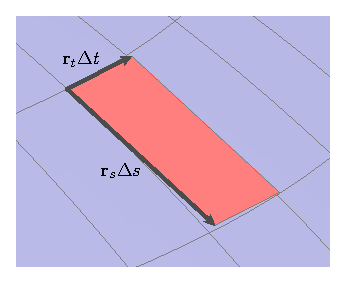
\includegraphics{figures/fig_11_6_approx.eps}
  \end{center}
  \caption{Approximation surface area with a parallelogram.}
  \label{F:11.6.approx}
\end{figure}

Say that the small parallelogram has area $S_{ij}$.  If we can find its area, then all that remains is to sum the areas of all of the generated parallelograms and take a limit.  Recall from our earlier work in the course that given two vectors $\vu$ and $\vv$, the area of the parallelogram spanned by $\vu$ and $\vv$ is given by the magnitude of their cross product, $| \vu \times \vv|$.  In the present context, it follows that the area, $S_{ij}$, of the parallelogram determined by the vectors $\vr_s(s_{i-1},t_{j-1}) \Delta s$ and $\vr_t(s_{i-1},t_{j-1}) \Delta t$ is
\begin{equation} \label{eq:11.6.parallelogram_area}
S_{ij} = |(\vr_s(s_{i-1},t_{j-1}) \Delta s) \times (\vr_t(s_{i-1},t_{j-1}) \Delta t)| = |\vr_s(s_{i-1},t_{j-1}) \times \vr_t(s_{i-1},t_{j-1})| \Delta s \Delta t,
\end{equation}
where the latter equality holds from standard properties of the cross product and length.

%\begin{activity} \label{A:11.6.3} Explain why the area of the parallelogram determined by the vectors $\vr_s(s_{i-1},t_{j-1}) \Delta s$ and $\vr_t(s_{i-1},t_{j-1}) \Delta t$ is
\begin{equation} \label{eq:11.6.parallelogram_area}
|(\vr_s(s_{i-1},t_{j-1}) \Delta s) \times (\vr_t(s_{i-1},t_{j-1}) \Delta t)| = |\vr_s(s_{i-1},t_{j-1}) \times \vr_t(s_{i-1},t_{j-1})| \Delta s \Delta t.
\end{equation}

\end{activity}
\begin{smallhint}

\end{smallhint}
\begin{bighint}

\end{bighint}
\begin{activitySolution}
Recall that the area of a parallelogram determined by the vectors $\vu$ and $\vv$ is $| \vu \times \vv|$. So the area of the parallelogram determined by the vectors $\vr_s(s_{i-1},t_{j-1}) \Delta s$ and $\vr_t(s_{i-1},t_{j-1}) \Delta t$ is
\[|(\vr_s(s_{i-1},t_{j-1}) \Delta s) \times (\vr_t(s_{i-1},t_{j-1}) \Delta t)|.\]
Now $\Delta s$ and $\Delta t$ are positive constants, so properties of the cross product show that 
\[|(\vr_s(s_{i-1},t_{j-1}) \Delta s) \times (\vr_t(s_{i-1},t_{j-1}) \Delta t)| = |\vr_s(s_{i-1},t_{j-1}) \times \vr_t(s_{i-1},t_{j-1})| \Delta s \Delta t.\]
\end{activitySolution}
\aftera


We sum the surface area approximations from Equation~(\ref{eq:11.6.parallelogram_area}) over all sub-rectangles to obtain an estimate for the total surface area, $S$, given by 
\[S \approx \sum_{i=1}^m \sum_{j=1}^n |\vr_s(s_{i-1},t_{j-1}) \times \vr_t(s_{i-1},t_{j-1})| \Delta s \Delta t.\] 
Taking the limit as $m, n \to \infty$ shows that the surface area of the surface defined by $\vr$ over the domain $D$ is given as follows.
%\[S = \lim_{m,n \to \infty} \sum_{i=1}^m \sum_{j=1}^n |\vr_s(s_{i-1},t_{j-1}) \times \vr_t(s_{i-1},t_{j-1})| \Delta s \Delta t = \iint_D |\vr_s \times \vr_t| \ dA.\]

\vspace*{5pt}
\nin \framebox{\hspace*{3 pt}
\parbox{6.25 in}{Let $\vr(s,t) = \langle x(s,t), y(s,t), z(s,t) \rangle$ be a parameterization of a smooth surface over a domain $D$. The \textbf{area of the surface}\index{surface area} defined by $\vr$ on $D$ is given by
\begin{equation} \label{E:surface_area}
S = \iint_D |\vr_s \times \vr_t | \ dA.
\end{equation}
} \hspace*{3 pt}}
\vspace*{5pt}

\begin{activity} \label{A:11.6.4} Consider the cylinder with radius $a$ and height $h$ defined parametrically by
\[\vr(s,t) = a\cos(s) \vi + a\sin(s) \vj + t \vk\]
for $0 \leq s \leq 2\pi$ and $0 \leq t \leq h$, as shown in Figure \ref{F:11.6.SA_cylinder_ex}.
\begin{figure}[h]
\begin{center}
%\resizebox{!}{2.0in}{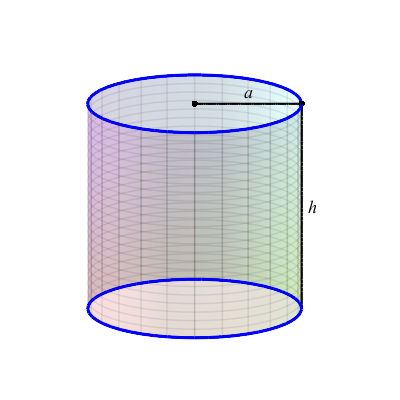
\includegraphics[trim=2cm 2cm 2cm 2cm, clip]{11_6_SA_cylinder}}
  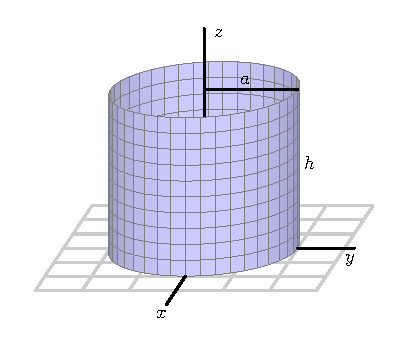
\includegraphics{figures/fig_11_6_cylinder.eps}
\end{center}
\caption{A cylinder.}
\label{F:11.6.SA_cylinder_ex}
\end{figure}
	\ba
	\item Set up an iterated integral to determine the surface area of this cylinder.
	
	\item Evaluate the iterated integral. 
	
	\item Recall that one way to think about the surface area of a cylinder is to cut the cylinder horizontally and find the perimeter of the resulting cross sectional circle, then multiply by the height.  Calculate the surface area of the given cylinder using this alternate approach, and compare your work in (b).

	\ea

\end{activity}
\begin{smallhint}

\end{smallhint}
\begin{bighint}

\end{bighint}
\begin{activitySolution}
\ba
\item We have 
\[\vr_s(s,t) = -a\sin(s) \vi + a\cos(s) \vj  \ \text{ and } \ \vr_t(s,t) = \vk,\]
so the area of the surface of the cylinder is 
\[\int \int_D |\vr_s \times \vr_t| \, dA = \int \int_D a \, dA.\]
In this case, $dA = ds \ dt$, so an iterated integral that represents the area of the surface is 
\[\int \int_D |\vr_s \times \vr_t| \, dA = \int_{0}^{h} \int_{0}^{2 \pi} a \, ds \, dt.\]

\item We can find the surface area of the cylinder by multiplying the circumference of the circle of radius $a$ by the height $h$ to obtain $2 \pi a h$. Evaluating the iterated integral yields
\begin{align*}
\int_{0}^{h} \int_{0}^{2 \pi} a^2 \, ds \, dt &= a \int_{0}^{h} \left. s \right|_{0}^{2 \pi}  \, dt \\
	&= 2 \pi a \int_{0}^{h}  \, dt \\
	&= 2 \pi a \left. t \right|_{0}^{h}  \\
	&= 2 \pi a h.
\end{align*}

\item If we slice the cylinder horizontally, a cross section is a circle of radius $a$. The circumference of this circle is $2 \pi a$. We multiply by the height of the cylinder to obtain the surface area as $2 \pi a h$ as expected. 
\ea
\end{activitySolution}
\aftera



%\begin{activity} \label{A:11.6.5} Set up an iterated integral to find the surface area of a sphere of radius $R$ (see Activity \ref{A:11.6.10}). Then calculate the surface area and compare to the formula for the surface area of sphere that you can find on-line. (Hint: Exploit the symmetry.)

\end{activity}
\begin{smallhint}

\end{smallhint}
\begin{bighint}

\end{bighint}
\begin{activitySolution}
From Activity \ref{A:11.6.1} we know that a parameterization of a sphere of radius $a$ centered at the origin is 
\[x(s,t) = a \cos(s) \cos(t), \ y(s,t) = a \sin(s) \cos(t), \ \text{ and } \ z(s,t) = a \sin(t)\]
for $s$ and $t$ in $[0, 2 \pi]$. By symmetry, we can just calculate the surface area of the sphere in the first octant, then multiply by 8. So we can assume $0 \leq s \leq \frac{\pi}{2}$, Now
\begin{align*}
\vr(s,t) &= \langle a\cos(s) \cos(t), a\sin(s)\cos(t), a\sin(t) \rangle, \\
\vr_s(s,t) &= \langle -a\sin(s) \cos(t), a\cos(s)\cos(t), 0 \rangle, \\
\vr_t(s,t) &= \langle -a\cos(s) \sin(t), -a\sin(s)\sin(t), -a\cos(t) \rangle,
\end{align*}
so
\begin{align*}
\lvert \vr_s(s,t) \times \vr_t(s,t) \rvert &= \lvert \langle -a\sin(s) \cos(t), a\cos(s)\cos(t), 0 \rangle \times \langle -a\cos(s) \sin(t), -a\sin(s)\sin(t), -a\cos(t) \rangle \rvert \\
    &= \lvert \langle -a^2\cos(s)\cos^2(t), -a^2\sin(s)\cos^2(t), a^2\cos(t)\sin(t) \rangle \rvert \\
    &= \sqrt{a^4\cos^2(s)\cos^4(t) + a^4\sin^2(s)\cos^4(t) + a^4\cos^2(t)\sin^2(t)} \\
    &= a^2\sqrt{\cos^2(t)} \\
    &= a^2\cos(t).
\end{align*}
Therefore, the surface area of this sphere is
\begin{align*}
8 \int_0^{\pi/2} \int_0^{\pi/2} a^2 \cos(t) \, dt \, ds &= 8a^2 \int_0^{\pi/2} \sin(t) \biggm|_0^{\pi/2} \, ds \\
    &= 8a^2 \int_0^{\pi/2} 1 \, ds \\
    &= 4\pi a^2.
\end{align*}

\end{activitySolution}
\aftera



As we noted earlier, we can take any surface $z = f(x,y)$ and generate a corresponding parameterization for the surface by writing $\langle s, t, f(s,t) \rangle$.    Hence, we can use our recent work with parametrically defined surfaces to find the surface area that is generated by a function $f = f(x,y)$ over a given domain.

\begin{activity} \label{A:11.6.6} Let $z = f(x,y)$ define a smooth surface, and consider the corresponding parameterization $\vr(s,t) = \langle s, t, f(s,t) \rangle$.
    \ba
    \item Let $D$ be a region in the domain of $f$.  Using Equation~\ref{E:surface_area}, show that the area, $S$, of the surface defined by the graph of $f$ over $D$ is
\[S = \iint_D \sqrt{\left(f_x(x,y)\right)^2 + \left(f_y(x,y)\right)^2 + 1} \ dA.\]

    \item Use the formula developed in (a) to calculate the area of the surface defined by $f(x,y) = \sqrt{4-x^2}$ over the rectangle $D = [-2,2] \times [0,3]$. 

    \item Observe that the surface of the solid describe in (b) is half of a circular cylinder.  Use the standard formula for the surface area of a cylinder to calculate the surface area in a different way, and compare your result from (b).

\ea

\end{activity}
\begin{smallhint}

\end{smallhint}
\begin{bighint}

\end{bighint}
\begin{activitySolution}
    \ba 
\item Recall that any surface defined by a function $f = f(x,y)$ in Cartesian coordinates can be thought of as a surface defined parametrically with parameters $s$ and $t$ by
\[x(s,t)=s, \ \ \ \ y(s,t) = t, \ \ \ \ \text{ and } \ \ \ \ z = f(s,t).\]
The surface is then given by the vector-valued function $\vr$ with $\vr(s,t) = \langle s, t, f(s,t) \rangle$. In this case we have
\[\vr_s(s,t) = \langle 1,0,f_s(s,t)\rangle \ \ \ \ \text{ and } \ \ \ \ \vr_t(s,t) = \langle 0,1,f_t(s,t)\rangle.\]
So
\[\lvert \vr_s \times \vr_t \rvert = \lvert \langle -f_s(s,t), -f_t(s,t), 1 \rangle \rvert = \sqrt{f_s(s,t)^2 + f_t(s,t)^2+1},\]
and the formula for surface area becomes
\[\int \int_D \sqrt{\left(f_x(x,y)\right)^2 + \left(f_y(x,y)\right)^2 + 1} \ dA.\]


    \item Using the formula from part (a) we have that the surface area is
\begin{align*}
\int_{-2}^2 \int_0^3 \sqrt{\left(-x(4-x^2)^{-1/2}\right)^2 + 0^2 + 1} \, dy \, dx &= \int_{-2}^2 \int_0^3 \sqrt{\frac{x^2}{4-x^2}+1} \, dy \, dx \\
    &= \int_{-2}^2 \int_0^3 \frac{2}{\sqrt{4-x^2}} \, dy \, dx \\
    &= \int_{-2}^2 \int_0^3  \frac{2}{\sqrt{4-x^2}}y\biggm|_0^3 \, dx \\
    &= 6\int_{-2}^2 \frac{1}{\sqrt{4-x^2}} \, dx \\
    &= 6 \arcsin{\frac{x}{2}}\biggm|_{-2}^2  \\
    &= 6\left(\arcsin(1)-\arcsin(-1)\right) \\
    &= 6\pi.
\end{align*}

\item The cross sections of the surface of this solid are semicircles with radius 2. So the surface area of this solid should be $2\pi \times 3 = 6\pi$.


\ea

\end{activitySolution}

\aftera


\begin{summary}
\item A parameterization of a curve describes the coordinates of a point on the curve in terms of a single parameter $t$, while a parameterization of a surface describes the coordinates of points on the surface in terms of two independent parameters.
\item If $\vr(s,t) = \langle x(s,t), y(s,t), z(s,t) \rangle$ describes a smooth surface in 3-space on a domain $D$, then the area, $S$, of that surface is given by
\[S = \iint_D |\vr_s \times \vr_t| \ dA.\]
\end{summary}


\nin \hrulefill

\newpage

\begin{exercises} 

\item Consider the ellipsoid given by the equation 
$$\frac{x^2}{16} + \frac{y^2}{25} + \frac{z^2}{9} = 1.$$
In Activity~\ref{A:11.6.10}, we found that a parameterization of the sphere $S$ of radius $R$ centered at the origin is 
\[x(r,s) = R\cos(s) \cos(t), \ y(s,t) = R \cos(s) \sin(t), \ \text{ and } \ z(s,t) = R\sin(s)\]
for $-\frac{\pi}{2} \leq s \leq \frac{\pi}{2}$ and $0 \leq t \leq 2\pi$.
	
\ba
	\item Let $(x,y,z)$ be a point on the ellipsoid and let $X = \frac{x}{4}$, $Y = \frac{y}{5}$, and $Z = \frac{z}{3}$. Show that $(X,Y,Z)$ lies on the sphere $S$. Hence, find a parameterization of $S$ in terms of $X$, $Y$, and $Z$ as functions of $s$ and $t$. 
	\item Use the result of part (a) to find a parameterization of the ellipse in terms of $x$, $y$, and $z$ as functions of $s$ and $t$. Check your parametrization by substituting $x$, $y$, and $z$ into the equation of the ellipsoid. Then check your work by plotting the surface defined by your parameterization with
    appropriate technology\footnote{e.g.,
    \url{http://web.monroecc.edu/manila/webfiles/calcNSF/JavaCode/CalcPlot3D.htm}
    or
    \url{http://www.flashandmath.com/mathlets/multicalc/paramrec/surf_graph_rectan.html}}.
\ea

\begin{exerciseSolution}
\ba
	\item If $(x,y,z)$ lies on the ellipse and $X = \frac{x}{4}$, $Y = \frac{y}{5}$, and $Z = \frac{z}{3}$, then 
\begin{align*}
X^2+Y^2+Z^2 &= \left(\frac{x}{4}\right)^2 + \left(\frac{y}{5}\right)^2 + \left(\frac{z}{3}\right)^2 \\
	&= \frac{x^2}{16} + \frac{y^2}{25} + \frac{z^2}{9} \\
	&= 1.
\end{align*}
So $(X,Y,Z)$ lies on the sphere $S$ and $S$ has parameterization 
\[X(r,s) = \cos(s) \cos(t), \ Y(s,t) = \cos(s) \sin(t), \ \text{ and } \ Z(s,t) = \sin(s)\]
for $-\frac{\pi}{2} \leq s \leq \frac{\pi}{2}$ and $0 \leq t \leq 2\pi$.
	\item Since $x = 4X$, $y = 5Y$, and $z = 3Z$ we have 
\[x(r,s) = 4\cos(s) \cos(t), \ y(s,t) = 5\cos(s) \sin(t), \ \text{ and } \ z(s,t) = 3\sin(s)\]
for $-\frac{\pi}{2} \leq s \leq \frac{\pi}{2}$ and $0 \leq t \leq 2\pi$. Note that 
\begin{align*}
\frac{x^2}{16} + \frac{y^2}{25} + \frac{z^2}{9} &= \cos^2(s)\cos^2(t) + \cos^2(s) \sin^2(t)  + \sin^2(s) \\
	&= \cos^2(s)[\cos^2(t) + \sin^2(t)] + \sin^2(s) \\
	&= \cos^2(s) + \sin^2(s) \\
	&= 1.
\end{align*}
So $x(r,s) = 4\cos(s) \cos(t)$, $y(s,t) = 5\cos(s) \sin(t)$, and $z(s,t) = 3sin(s)$ is a parametrization of the ellipse. 
\ea
\end{exerciseSolution}

  \item In this exercise, we explore how to use a parametrization and iterated integral to determine the surface area of a sphere.
  \ba
  	\item Set up an iterated integral whose value is the portion of the surface area of a sphere of radius $R$ that lies in the first octant (see the parameterization you developed in Activity \ref{A:11.6.10}). 
	\item Then, evaluate the integral to calculate the surface area of this portion of the sphere.
	\item By what constant must you multiply the value determined in (b) in order to find the total surface area of the entire sphere.  	
\item Finally, compare your result to the standard formula for the surface area of sphere. 
  \ea

\begin{exerciseSolution}
\ba
\item From Activity \ref{A:11.6.10} we know that a parameterization of a sphere of radius $R$ centered at the origin is 
\[x(s,t) = R \cos(s) \cos(t), \ y(s,t) = R\sin(s) \cos(t), \ \text{ and } \ z(s,t) = R \sin(t)\]
for $-\frac{\pi}{2} \leq s \leq \frac{\pi}{2}$ and $t$ in $[0, 2 \pi]$. By symmetry, we can just calculate the surface area of the sphere in the first octant, then multiply by 8. So we can assume $0 \leq s, t \leq \frac{\pi}{2}$.
\item With $\vr(s,t) = \langle R \cos(s) \cos(t),  R\sin(s) \cos(t),  R \sin(t) \rangle$ we have
\begin{align*}
\vr_s(s,t) &= \langle -R\sin(s) \cos(t), R\cos(s)\cos(t), 0 \rangle, \\
\vr_t(s,t) &= \langle -R\cos(s) \sin(t), -R\sin(s)\sin(t), -R\cos(t) \rangle,
\end{align*}
and so 
\begin{align*}
\lvert \vr_s(s,t) \times \vr_t(s,t) \rvert &= \lvert \langle -R\sin(s) \cos(t), R\cos(s)\cos(t), 0 \rangle \times \langle -R\cos(s) \sin(t), -R\sin(s)\sin(t), -R\cos(t) \rangle \rvert \\
    &= \lvert \langle -R^2\cos(s)\cos^2(t), -R^2\sin(s)\cos^2(t), R^2\cos(t)\sin(t) \rangle \rvert \\
    &= \sqrt{R^4\cos^2(s)\cos^4(t) + R^4\sin^2(s)\cos^4(t) + R^4\cos^2(t)\sin^2(t)} \\
    &= R^2\sqrt{\cos^2(t)} \\
    &= R^2\cos(t).
\end{align*}
Therefore, the surface area of the first octant portion of the sphere is
\begin{align*}
 \int_0^{\pi/2} \int_0^{\pi/2} R^2 \cos(t) \, dt \, ds &= 8R^2 \int_0^{\pi/2} \sin(t) \biggm|_0^{\pi/2} \, ds \\
    &= R^2 \int_0^{\pi/2} 1 \, ds \\
    &= \frac{1}{2}\pi R^2.
\end{align*}
\item We multiply the previous result by 8 to reproduce the surface area calculation in each of the eight octants. So the surface area of a sphere of radius $R$ is $4 \pi R^2$. 
\item  The result of part (c) is the standard formula for the surface area of a sphere of radius $R$. 
\ea
\end{exerciseSolution}

\item Consider the plane generated by $z = f(x,y) = 24 - 2x - 3y$ over the region $D = [0,2]\times[0,3]$.
	
\ba
	\item Sketch a picture of the overall solid generated by the plane over the given domain.
	\item Determine a parameterization $\vr(s,t)$ for the plane over the domain $D$.
	\item Use Equation~\ref{E:surface_area} to determine the surface area generated by $f$ over the domain $D$.
	\item Observe that the vector $\vu = \langle 2, 0, -4 \rangle$ points from $(0,0,24)$ to $(2,0,20)$ along one side of the surface generated by the plane $f$ over $D$.  Find the vector $\vv$ such that $\vu$ and $\vv$ together span the parallelogram that represents the surface defined by $f$ over $D$, and hence compute $| \vu \times \vv |$.  What do you observe about the value you find?
\ea

\begin{exerciseSolution}
\ba
	\item The solid looks like a box with a slanted top. 
	\item If we let $x(s,t) = s$ and $y(s,t) = t$, then $z(s,t) = 24-2s-3t$ provides a parameterization of the plane. So we can let $\vr(s,t) = s \vi + t \vj + (24-2s-3t) \vk$. 
	\item In our situation we have $\vr_s(s,t) = \vi - 2 \vk$ and $\vr_t(s,t) = \vj - 3 \vk$. So $\vr_s(s,t) \times \vr_t(s,t) = 2 \vi + 3\vj + \vk$. So  the surface area generated by $f$ over the domain $D$ is found by 
\begin{align*}
 \int_0^{3} \int_0^{2} | \langle 2,3,1 \rangle | \, dt \, ds &=  \sqrt{14} \int_0^{3} \int_0^{2} \, dt \, ds \\
    &= 6 \sqrt{14}.
\end{align*}
	\item Take $\vv = \langle 0, 2, -9 \rangle$ to be the vector that points from $(0,0,24)$ to $(0,3,15)$ along one side of the surface generated by the plane $f$ over $D$. Then $\vu$ and $\vv$ together span the parallelogram that represents the surface defined by $f$ over $D$. Here we have 
\[| \vu \times \vv | = | \langle 12, 18, 6 \rangle | = \sqrt{504} = 6 \sqrt{14}.\]
Since $| \vu \times \vv |$ is the area of the parallelogram determined by $\vu$ and $\vv$, we should expect this area to be the same as the surface area of the surface defined by the plane $f$ over $D$. 
\ea
\end{exerciseSolution}

\item A cone with base radius $a$ and height $h$ can be realized as the surface defined by $z = \frac{h}{a} \sqrt{x^2+y^2}$, where $a$ and $h$ are positive.  
 	\ba
	\item Find a parameterization of the cone described by $z = \frac{h}{a} \sqrt{x^2+y^2}$. (Hint: Compare to the parameterization of a cylinder as seen in Activity  \ref{A:11.6.4}.) 
	
	\item Set up an iterated integral to determine the surface area of this cone.
	
	\item Evaluate the iterated integral to find a formula for the lateral surface area of a cone of height $h$ and base $a$. 
	
	\ea

\begin{exerciseSolution}
\ba
\item Let $t$ run along the positive $z$-axis from 0 to $h$. By similar triangles, the cross section of the cone at height $t$ parallel to the $x$-$y$ plane has radius $\frac{h}{a}t$. We can think of the cone as made of circles with these varying radii, so a parameterization of the cone is 
\[\vr(s,t) = \frac{h}{a}t \cos(s) \vi + \frac{h}{a}t \sin(s) \vj + t \vk,\]
for $0 \leq s \leq 2 \pi$ and $0 \leq t \leq a$. 

\item We have 
\[\vr_s(s,t) = -\frac{h}{a}t\sin(s) \vi + \frac{h}{a}t\cos(s) \vj  \ \text{ and } \ \vr_t(s,t) =  \frac{h}{a} \cos(s) \vi + \frac{h}{a} \sin(s) \vj + \vk,\]
and
\[\vr_s(s,t) \times \vr_t(s,t) = -\frac{h}{a}t\cos(s) \vi + \frac{h}{a}t\sin(s) \vj + \left(\frac{a}{h}\right)^2 t \vk.\]
By symmetry, we calculate the area of the cone in the first octant and multiply by 4 to obtain the area of the surface of the cone as
\[4\int_0^{\pi/2} \int_0^a |\vr_s \times \vr_t| \, dt \, ds = 4\int_0^{\pi/2} \int_0^a \frac{a}{h^2} \sqrt{h^2+a^2} t \, dt \, ds.\]

\item Evaluating the iterated integral yields
\begin{align*}
4\int_0^{\pi/2} \int_0^a \frac{a}{h^2} \sqrt{h^2+a^2} t \, dt \, ds &= 4\frac{a}{h^2} \sqrt{h^2+a^2} \int_0^{\pi/2} \frac{1}{2}t^2 \biggm|_0^h \, ds \\
	&= 2 a \sqrt{h^2+a^2} \int_{0}^{\pi/2}  \, ds \\
	&= \pi  a \sqrt{h^2+a^2}. 
\end{align*}

\ea
\end{exerciseSolution}
\end{exercises}
\afterexercises


\clearpage
